\documentclass{article}
\usepackage[utf8]{inputenc}
\usepackage[english]{babel}
\usepackage{amsmath}
\usepackage{natbib}
\usepackage{graphicx}
\usepackage{hyperref}
\usepackage{caption}
\usepackage{epstopdf}
\usepackage{float}
\epstopdfsetup{outdir=./}

\begin{document}

%\begin{center}

\begin{figure}
\centering

\includegraphics[width=2.25in]{munlogo.jpg}
\end{figure}


%\end{center}

{\centering


{\huge \bf Growing Degree Days}




\vspace{20mm} %5mm vertical space
\scshape % Small caps
CMSC 6950 - Computer Based Research Tools and Applications \\ [\baselineskip]
16th June, 2017 \\[\baselineskip] 
\vspace{20mm} %5mm vertical space
Prepared by \\[\baselineskip]
{\Large  Yasaman Bahrami Samani\\ Majid Beheshti Mohtasham \\Hoda Rafieipour  \\Frieda Samuel  \\Haris Tanvir  \\AbdAl Aziz Abusaleh  \\ \par}
\vfill
{\itshape \bf Memorial University of Newfoundland \par} 
}

\newpage

{\centering
  \section*{Abstract}
}

{\itshape In this work, we have worked on a heat index called Growing Degree Days (GDD). We have focused on three Canadian cities’ weather history in 2016. We have used the data of St. John's, Toronto, and Vancouver. It is clear that that they have different GDDs as they are located in different zones of this country. The first city in terms of highest GDD was Toronto with 1797  $^{\circ}$C. By contrast, the lowest amount belonged to the St. John's with 763  $^{\circ}$C. Finally, Vancouver with 1211  $^{\circ}$C was the second one. In this project, we did some analyses of GDD on the mentioned cities.\\
}



\section{ \bf Introduction}
The growing degree days (GDD) is a temperature index tool used in agriculture to predict the best planting season for a plant. GDD enhances predicting the best planting time of a crop to its maturity, in terms of high heat accumulated in the ground in regions conducive. GDD is used to predict and compare the growing rate of a plant from germination to yielding and predict future planting.
Mathematically, GDD is calculated using the following equation:


\begin{equation}
\textrm{GDD} = \left(\frac{T_{max} + T_{min}}{2}\right) - T_{base}
\label{eqn:gdd}
\end{equation}

\noindent 
Generally, GDD is calculated by adding the maximum (Tmax) and minimum (Tmin) temperature together dividing by two (2) and then subtracting the base temperature (Tbase). 
When determining the GDD of a plant, each plant has a conducive temperature for development and so it has a base temperature (Tbase). The base temperature is the lowest temperature a plant can survive in. (Tbase) will be consider to be 10 $^{\circ}$C for the calculation of GDD in this report.
GDD calculates temperature thus the unit for the measuring temperature is used which is in $^{\circ}$F or $^{\circ}$C. \\
The reference temperature for a given plant is the temperature below which its development slows or stops. For example, peas are planted during the cold season, where it has a reference temperature of 40  $^{\circ}$F while sweet corn and soybeans are planted during the hot season, where they have a reference temperature of 50 degrees  $^{\circ}$F.
Having calculated the GDD for the above cities suitable region will yield more plants when suitable crops are planted.
In this report, detailed results of GDD calculations will be presented. The GDD calculations were done including three main cities of Canada in 2016. In which they are St. John’s, Toronto, and Vancouver.



\section{ \bf Methodology}
\subsection{Data Collection}
Firstly, the GDD data for the main three cities have been obtained from the website: http://climate.weather.gc.ca. After that, the values of minimum and maximum daily temperatures have been extracted for the selected cities. Eventually, the values of daily GDD were calculated and the results in the shape of plots. Here we set temperature below Tbase to Tbase before calculating the average. And this instance happens when the daily mean temperature is lower than the base temperature which gives a zero value for GDD. 

\begin{itemize}
\item Downloading relevance data from the url which we provide as the input. 
\item Calculating Daily GDD for all of three cities. 
\item Computing Cumulative GDD for the selected periods.
\item Creating  plot to depict information in annual GDD . 
\item Creating  plot to show accumulated GDD vs time for the selected periods. 
\item Creating plot for demonstrating GDD vs mean temperature and Total precip.
\end{itemize}


\subsection{ \bf Minimum Core Tasks}

\begin{enumerate}
\item  Downloading the data from the defined url by a specific function automatically based on the city names and station IDs
\item  Showing annual cycle of min/max daily temperatures for selected Canadian cities(Fig. \ref{dd_min-max})
\begin{center}
\begin{figure}[H]
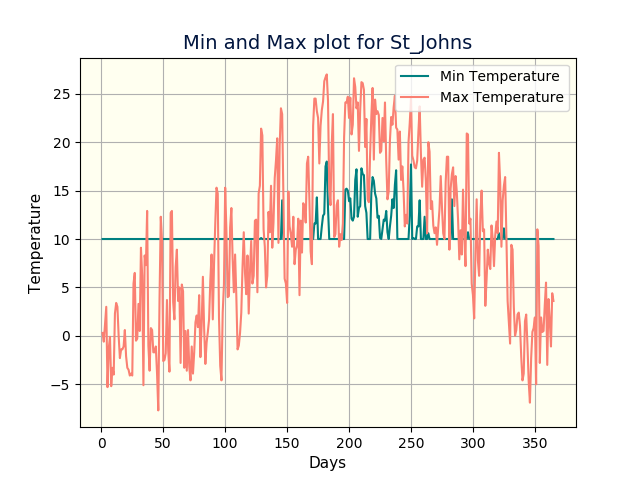
\includegraphics[width=3.25in]{minMaxPlotSt_Johns.png}

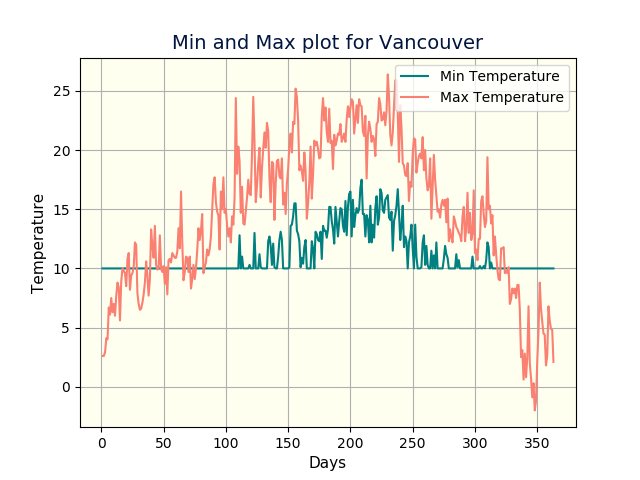
\includegraphics[width=3.25in]{minMaxPlotVancouver.png}

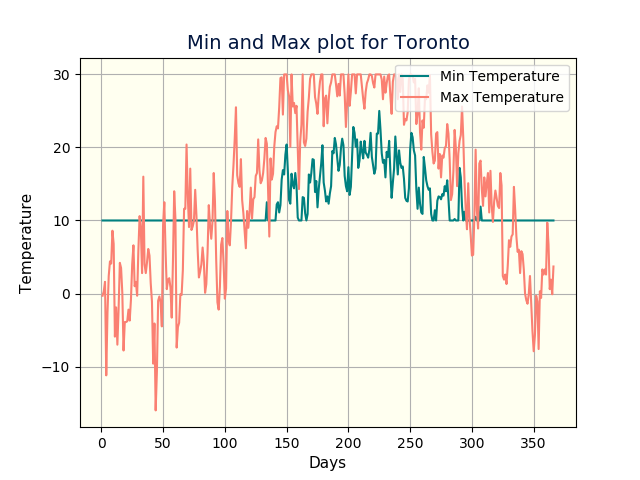
\includegraphics[width=3.25in]{minMaxPlotToronto.png}

\caption{Min/Max temps by 2016}
\label{gdd_min-max}
\end{figure}
\end{center}

\item Calculating and storing GDD to analyze via the command line(Fig. \ref{gdd_ann-cycle})
\item  Presenting accumulated GDD based on time for all the chosen cities by plot
\begin{center}
\begin{figure}[H]
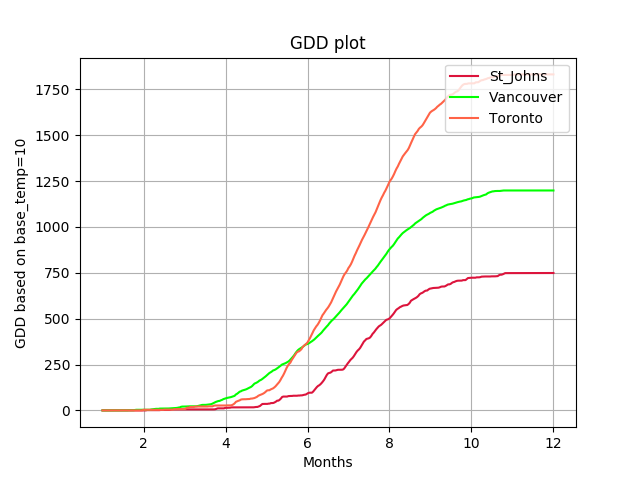
\includegraphics[width=3.25in]{GDDPlotIMG.png}
\caption{ Annual cumulative GDD 2016}
\label{gdd_ann-cycle}
\end{figure}
\end{center}

\end{enumerate}


\subsection{ \bf Secondary Tasks }
\begin{enumerate}
\item Bokeh plots to address GDD for the  chosen cities(Fig. \ref{bokeh_min-max})
\begin{center}
\begin{figure}[H] 
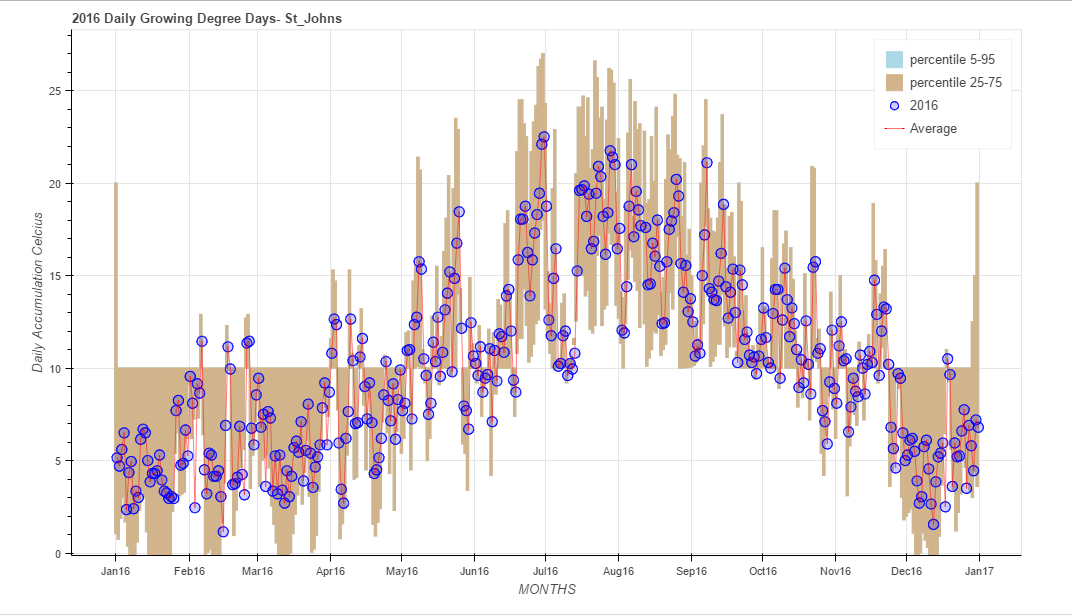
\includegraphics[width=3.25in]{secTask-1St_Johns.png}\\

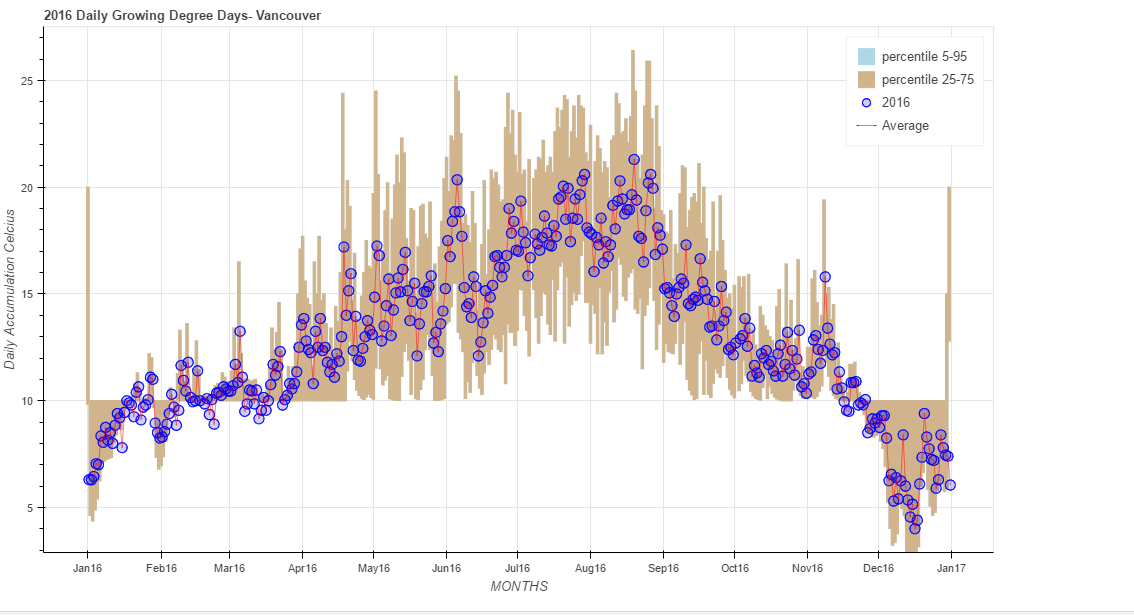
\includegraphics[width=3.25in]{secTask-1Vancouver.png}\\

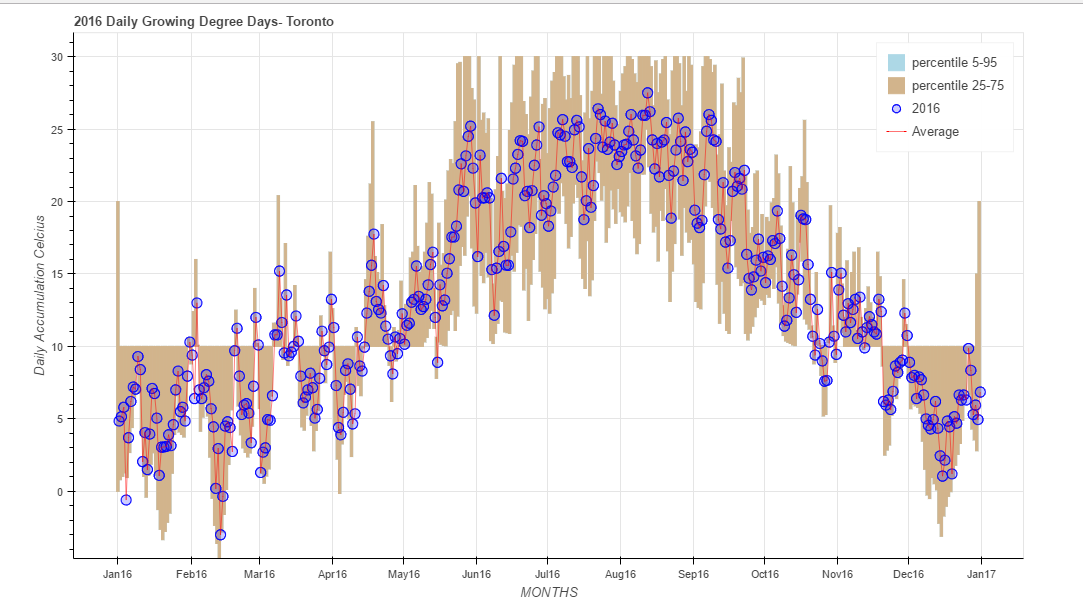
\includegraphics[width=3.25in]{secTask-1Toronto.png}\\

\caption{Bokeh plot for showing GDD min-max all the given cities}
\label{bokeh_min-max}
\end{figure}
\end{center}
\item Producing  a map to show effective GDD over  all the Canada(Fig. \ref{gdd_map})
\begin{center}
\begin{figure}[H]
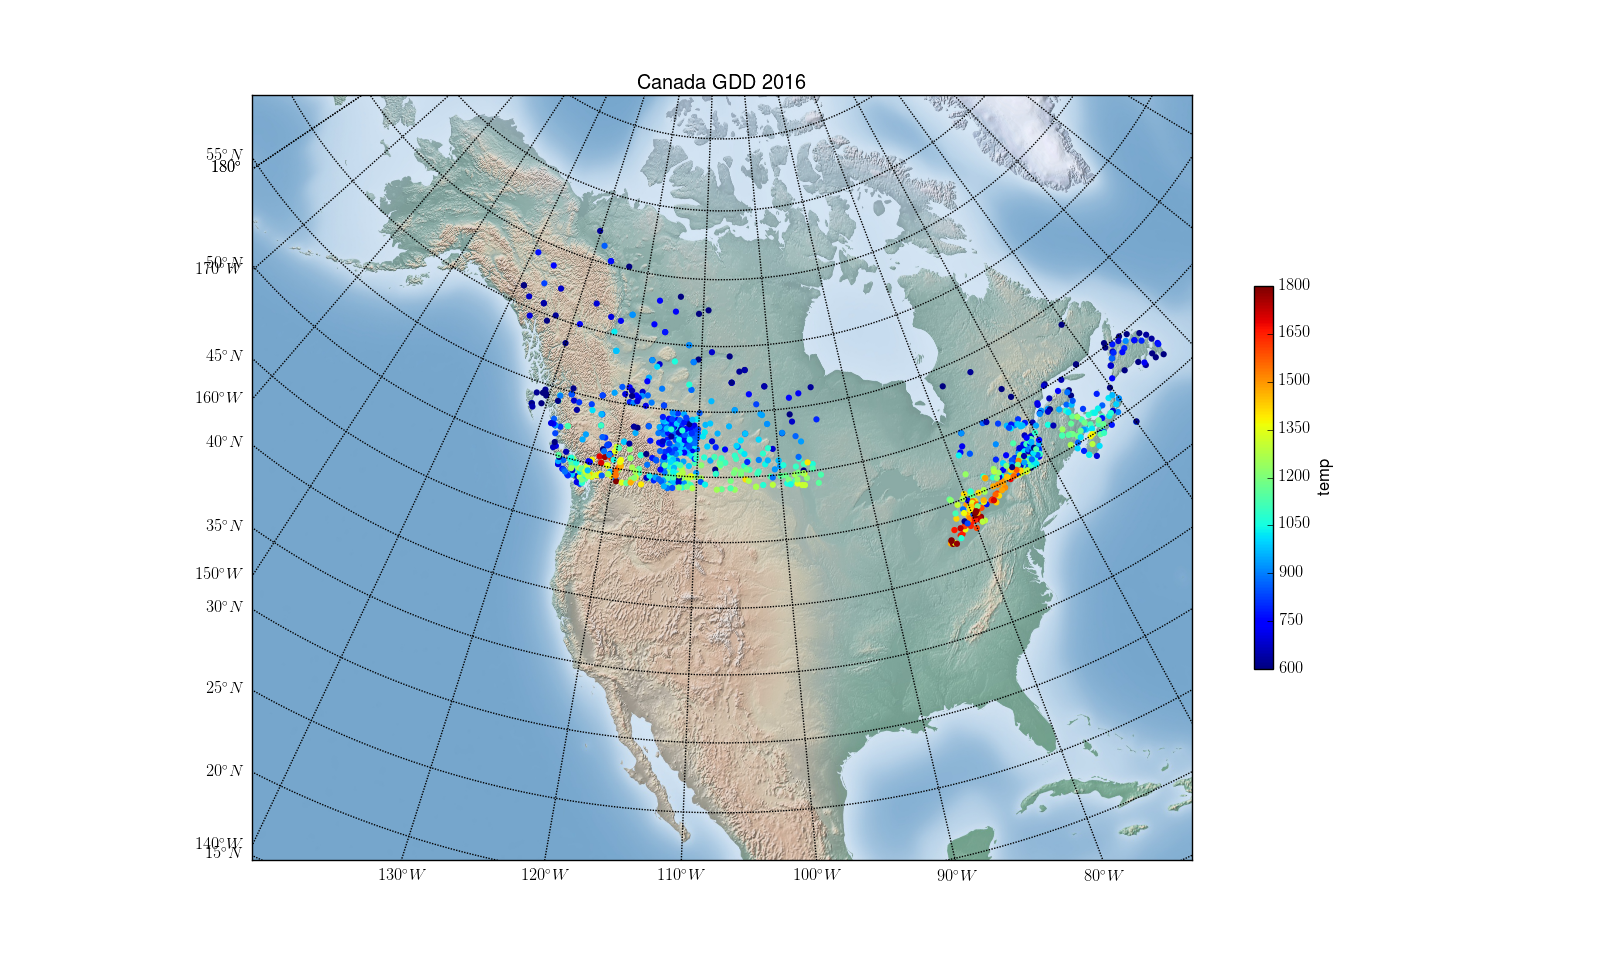
\includegraphics[width=4.25in]{map_shadedrelief.png}
\caption{GDD map situation in 2016}
\label{gdd_map}
\end{figure}
\end{center}
\item Presenting GDD calculation on different $T_{base}$s  varies in the ST John's(Fig. \ref{gdd_diff-tbase})
\begin{center}
\begin{figure}[H]
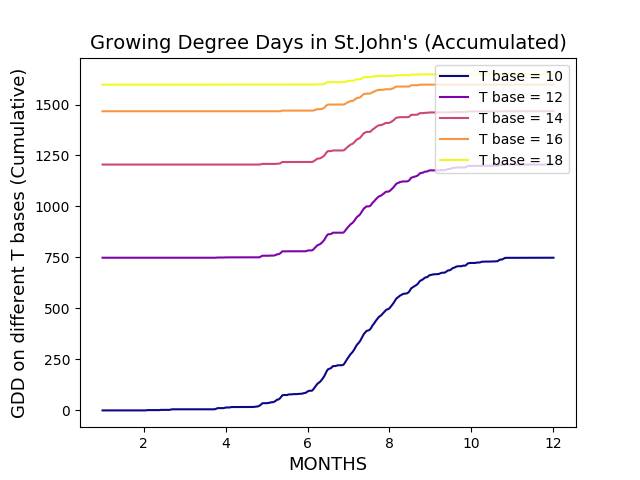
\includegraphics[width=4.25in]{secTask-3.png}
\caption{GDD dependencies to $T_{base}$ values in ST John's in 2016}
\label{gdd_diff-tbase}
\end{figure}
\end{center}

\item Standalone bokeh plots embeded in HTML presentation for interactive selection of data (Fig. \ref{gdd_interactive})
\begin{center}
\begin{figure}[H]
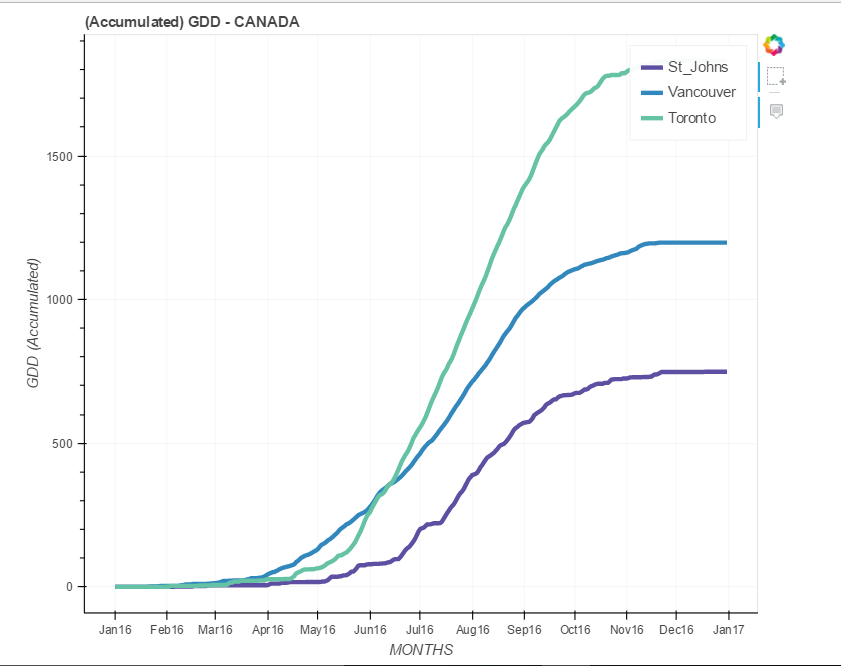
\includegraphics[width=3.95in]{secTask-4.png}
\caption{Interactive plot of accumulative GDD 2016}
\label{gdd_interactive}
\end{figure}
\end{center}

\item Bokeh server plot for visualization of accumulated GDD for ST John's (Fig. \ref{bokeh-server-plot_sj})

\begin{center}
\begin{figure}[H]
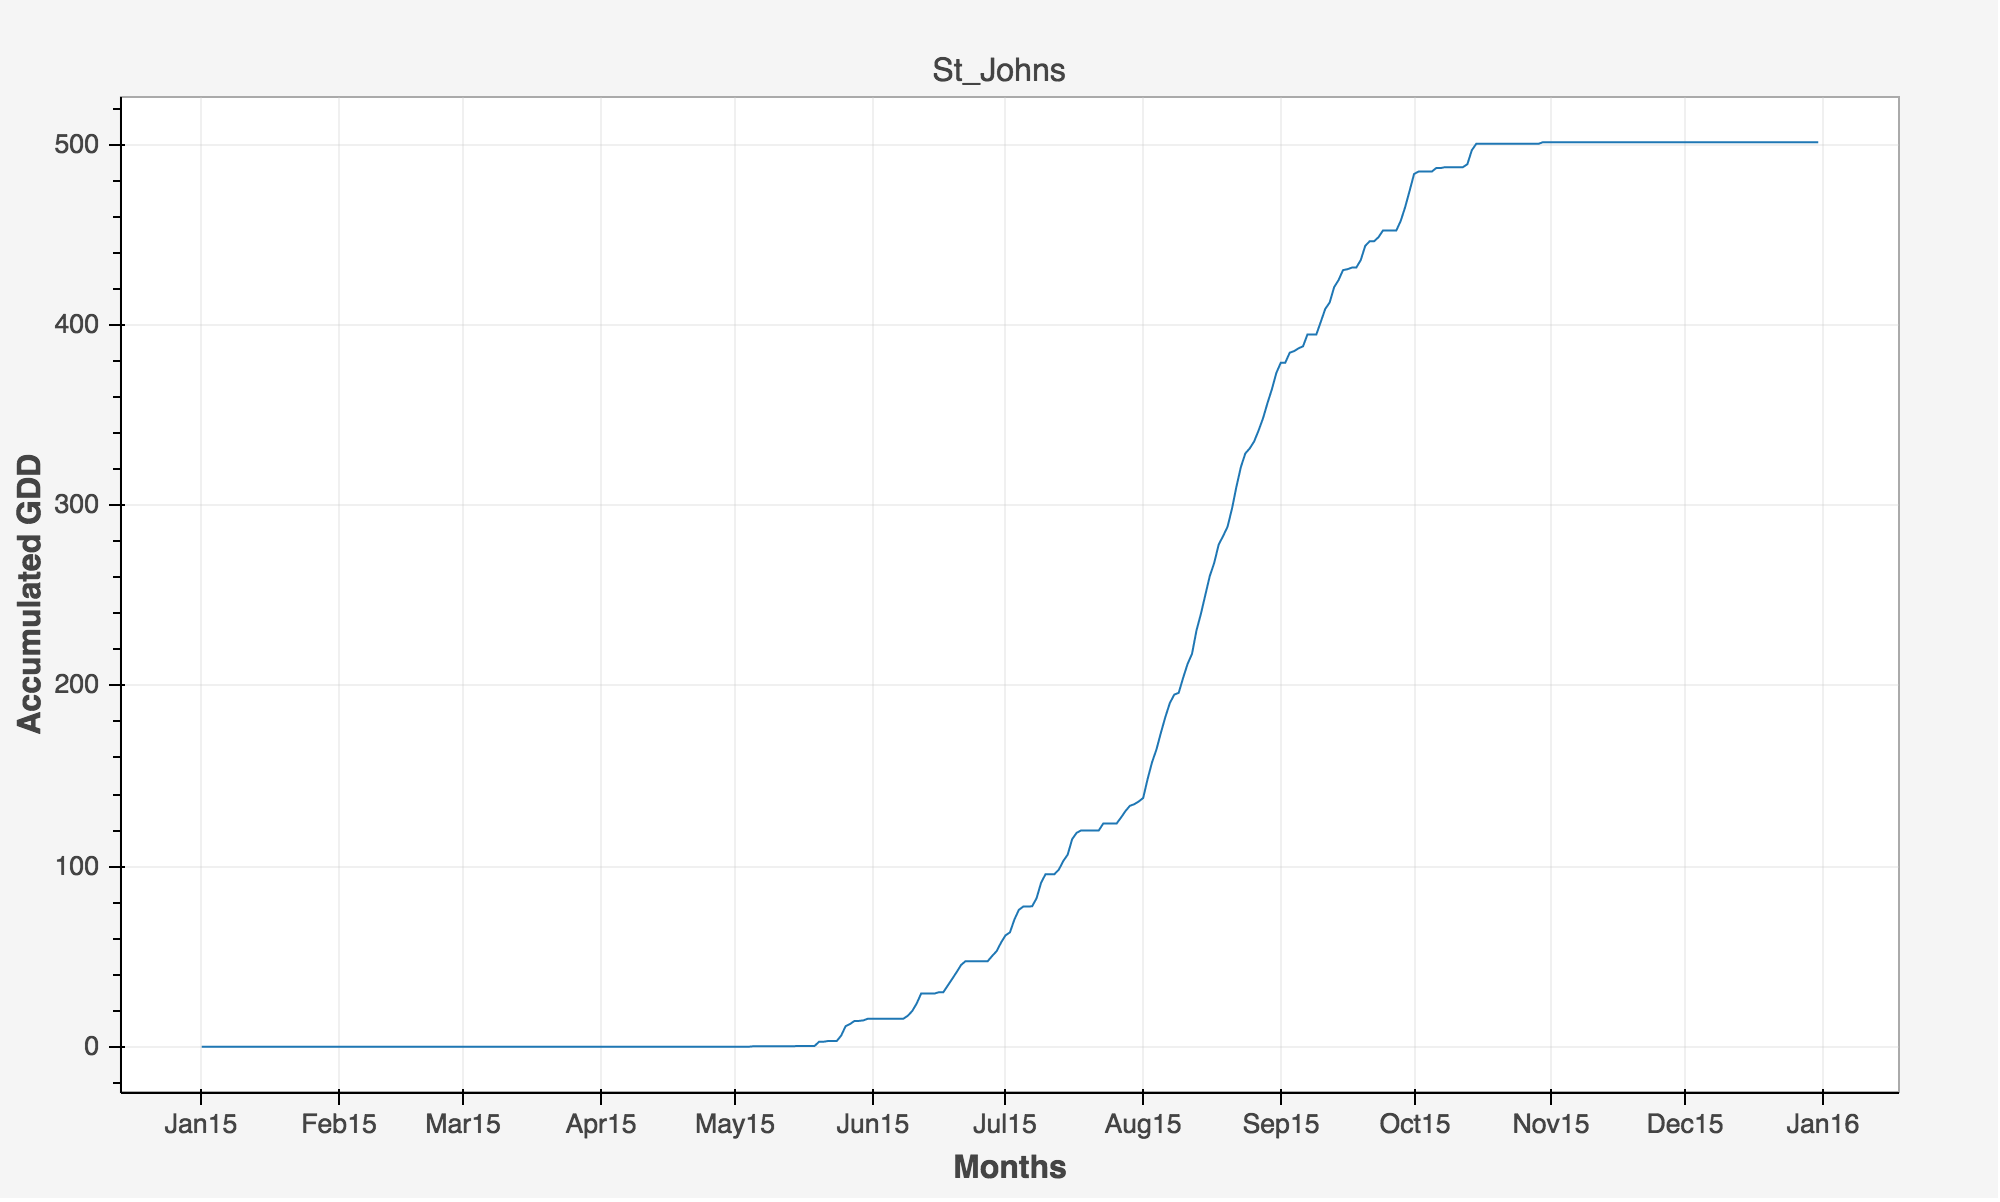
\includegraphics[width=4.25in]{secTask-5.png}
\caption{Bokeh server plot of cumulative GDD for St. John's in 2016}
\label{bokeh-server-plot_sj}
\end{figure}
\end{center}

\item Final task which is optional and shows the plots of changes of the mean temperature and total Precipitation over GDD (Fig. \ref{freeTask})
\begin{center}
\begin{figure}[H] 
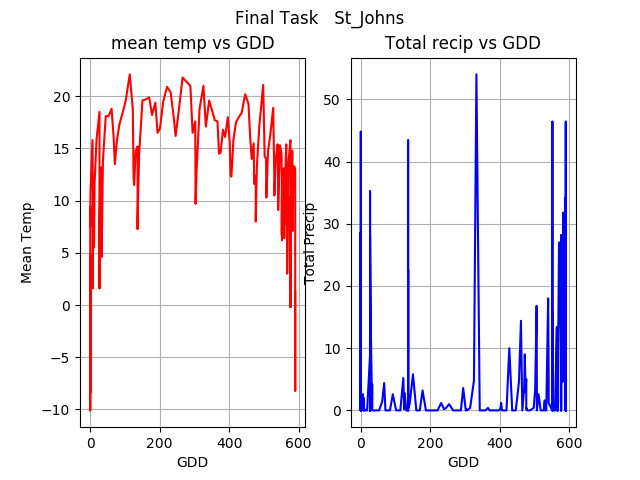
\includegraphics[width=3.25in]{finalTaskSt_Johns.png}\\

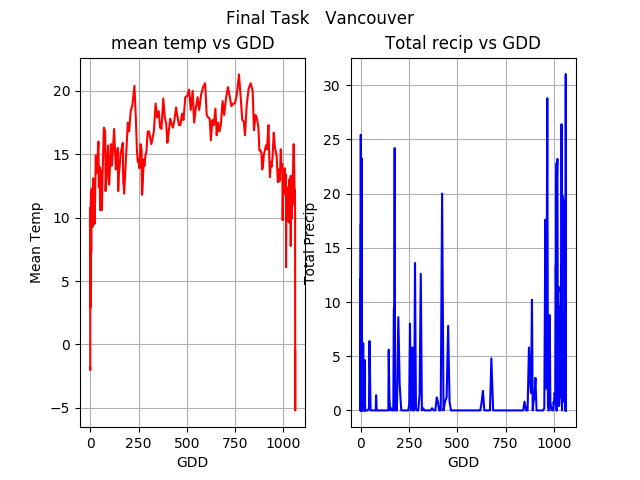
\includegraphics[width=3.25in]{finalTaskVancouver.png}\\

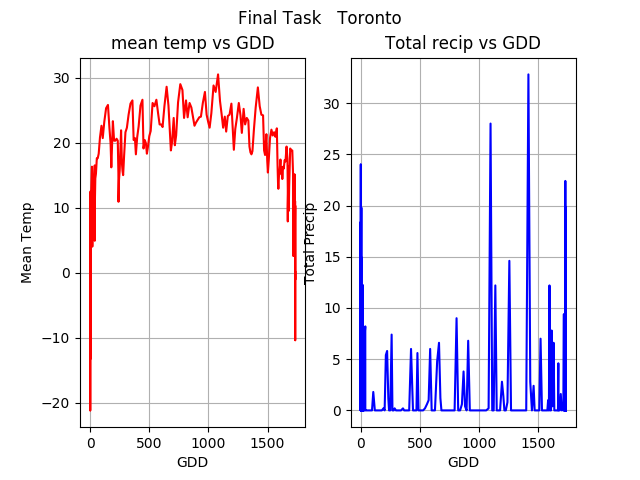
\includegraphics[width=3.25in]{finalTaskToronto.png}\\

\caption{Mean temp and total Precipitation over GDD}
\label{freeTask}
\end{figure}
\end{center}
\end{enumerate}





\section{Conclusion}
We have computed the GDD of ST John's, Vancouver, and Toronto by 2016. Accumulation GDD is an useful tool to compare the heat accumulation which is provided by summing of GDD. The final results and plots depict that Toronto, Vancouver and ST John's has the highest cumulative GDD respectively with the amounts of 1797, 1211, and 763 $^{\circ}$C.
 

\section{References}
%\bibliographystyle{plain}
\begin{enumerate}
\item McMaster, G.S., Smika, D.E.\textbf{1988} , Estimation and evaluation of winter wheat phenology in the central Great Plains. Agric. For. Meteorol. 43, 1-18
\item Masle, J., Doussinalut, G., Farquhar, G.D., Sun, B.\textbf{1989}, Foliar stage in wheat correlates better to photothermal time than tothermal time. \textit{Plant, Cell Environ}. 12, 235-247.
\item Wilhelm, W.W., McMaster, G.S., \textbf{1995}, The importance of the phyllochron in studying the development of grasses.  \textit{Crop Sci}. 35, 1-3.
\item \href{url}{$https://en.wikipedia.org/wiki/Growing_degree-day$}
\item \href{url}{$http://climate.weather.gc.ca$}

\end{enumerate}
\end{document}

%\bibliography{./reports/references.bib}



